\documentclass{beamer}

% Romanian Language support
\usepackage{ucs}
\usepackage[utf8x]{inputenc}
\PrerenderUnicode{aâîțșĂÎÂȚȘ}
\usepackage[english,romanian]{babel}

\usepackage{hyperref}   % use \url{http://$URL} or \href{http://$URL}{Name}
\usepackage{verbatim}
\usepackage{underscore} % underscores need not be escaped
\usepackage{booktabs}   % nice looking tables
\usepackage{array}      % column size options in tables
\usepackage[normalem]{ulem}       % for striketrough text

\mode<presentation>
%{ \usetheme{Berlin} }

% Disable useless navigation symbols.
\setbeamertemplate{navigation symbols}{}
\setbeamertemplate{footline}[frame number]

\title[Dig into iOS]{Dig into iOS Without Using an iOS Device}
\institute{PR204/ED217 Escape}
\author[Răzvan Deaconescu]{Răzvan Deaconescu \\
razvan.deaconescu@cs.pub.ro}
\date{November 4, 2016}

\begin{document}

\frame{\titlepage}

\begin{frame}{Why Hack the iPhone?}
  \begin{itemize}
    \pause \item Fun, Fame, Fortune
    \pause \item proprietary code, popularity, nice hacking community (\url{https://www.theiphonewiki.com/wiki/Main_Page})
    \pause \item CVEs: \url{http://lists.apple.com/archives/security-announce/2016/Oct/msg00000.html}
    \pause \item research papers (\textit{SandScout: Automatic Detection of Flaws in iOS Sandbox Profiles}, ACM CCS 2016)
    \pause \item Apple Bug Bounty: \url{https://techcrunch.com/2016/08/04/apple-announces-long-awaited-bug-bounty-program/}
  \end{itemize}
\end{frame}

\begin{frame}{iOS}
  \begin{figure}
    \centering
    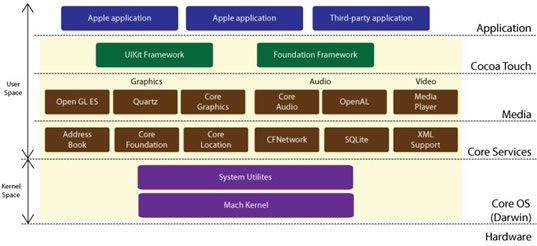
\includegraphics[width=\textwidth]{img/ios-architecture}
  \end{figure}
  \vspace{1cm}
  \centering
  \footnotesize{\url{http://blog.inf.ed.ac.uk/sapm/files/2014/02/blog_2.jpg}}
\end{frame}

\begin{frame}{iOS Security Features}
  \begin{itemize}
    \item \url{https://www.apple.com/business/docs/iOS_Security_Guide.pdf}
    \item Secure Boot
    \item Code Signing
    \item Sandboxing, Privacy Settings
    \item Extensions, Entitlements
  \end{itemize}
\end{frame}

\begin{frame}{Digging into iOS}
  \begin{itemize}
    \pause \item Apple documentation (poor)
    \pause \item community documentation (better)
    \pause \item build iOS apps using XCode, static + dynamic analysis (lldb)
    \pause \item jailbreak iOS device, do dynamic analysis
    \pause \item static analysis \textbf{without} using an iOS device
  \end{itemize}
\end{frame}

\begin{frame}{iOS Firmware Files}
  \begin{itemize}
    \item \textit{https://ipsw.me/}
    \item filesystem image, kernel image
    \item encrypted until iOS9; decrypt using firmware keys: \url{https://www.theiphonewiki.com/wiki/Firmware_Keys}
    \item not-encrypted after iOS10
  \end{itemize}
\end{frame}

\begin{frame}{Overview of Firmware Processing}
  \begin{figure}
    \centering
    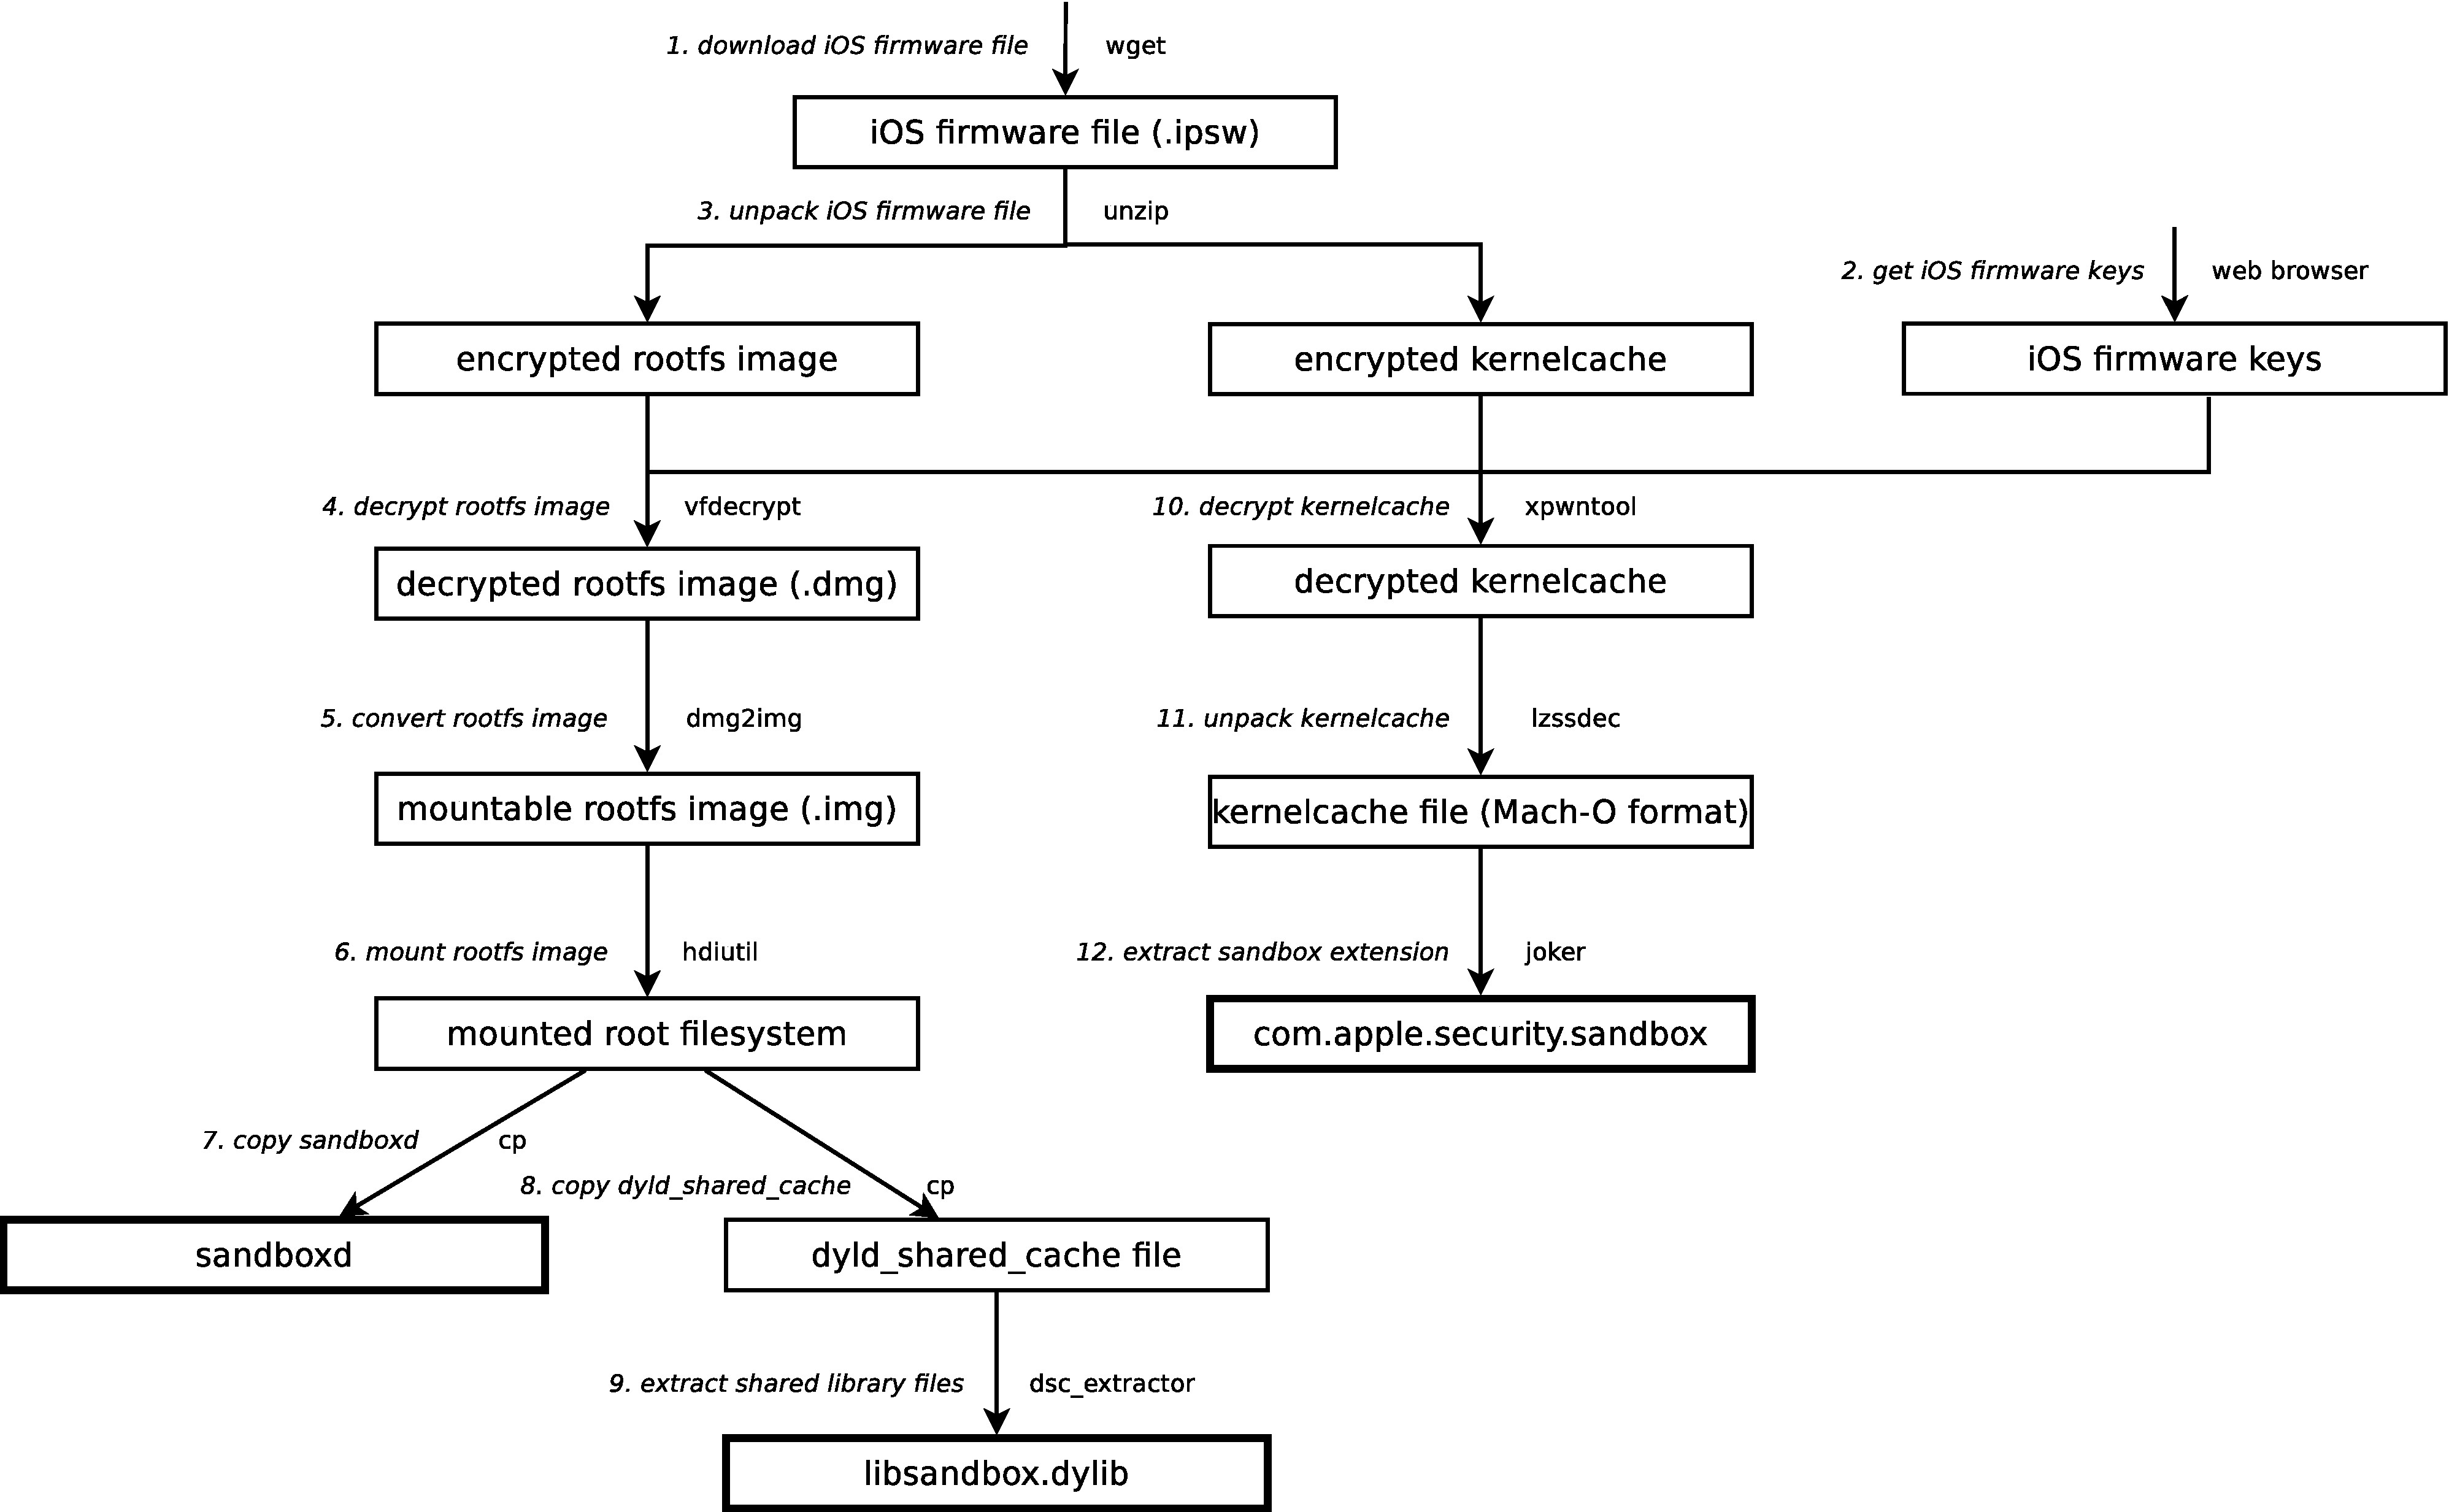
\includegraphics[width=\textwidth]{img/extract-required-files}
  \end{figure}
  \vspace{0.2cm}
  \centering
  \footnotesize{Deaconescu et al.: \textit{SandBlaster: Reversing the Apple Sandbox}, arXiv:1608.04303}
\end{frame}

\begin{frame}{Interesting Files}
  \begin{itemize}
    \pause \item kernel image
      \begin{itemize}
        \item kernel extensions (\textit{com.apple.sandbox})
        \item IOKit drivers in kernel image
      \end{itemize}
    \item \texttt{dyld_shared_cache}, library files
    \item Application executable files
    \item system daemons
  \end{itemize}
\end{frame}

\begin{frame}{Binary Inspection}
  \begin{itemize}
    \item static analysis: \texttt{otool}, IDA, MachO View
    \item reversing: \texttt{strings}, \texttt{hexdump}, scripting language, \texttt{ldid}
    \item use cases
      \begin{itemize}
        \item kernel inspection
        \item extract appplication entitlements
        \item security holes in executables
        \item \textbf{reverse the sandbox}
      \end{itemize}
  \end{itemize}
\end{frame}

\begin{frame}{Other Approaches}
  \begin{itemize}
    \item process and IPC investigation (jailbroken)
    \item debugging apps (jailbroken)
    \item decrypt and dump 3rd party apps (jailbroken)
    \item automatic download of 3rd party apps (Orikogbo et al.: \textit{CRiOS: Toward Large-Scale iOS Application Analysis}, SPSM 2016)
  \end{itemize}
\end{frame}

\begin{frame}{Objectives}
  \begin{itemize}
    \item find flaws in sandbox profiles: SandScout
    \item connect concepts, create jailbreak roadmap: iOracle
    \item find vulnerabilities (CVEs, bug bounty)
    \item help Apple security team improve product (business constraints vs. reported security issues)
    \item maybe in the future: deterministic rowhammer on iOS
    \item publish tools (SandBlaster, SandScout) as open source software
  \end{itemize}
\end{frame}

\begin{frame}{Takeaway}
  \begin{itemize}
    \item iOS is interesting and challenging: proprietary, incomplete knowledge base, good security features
    \item one can dig into iOS without an iOS device
    \item a (jailbroken) device is still required for testing/validation and dynamic analysis
  \end{itemize}
\end{frame}

\end{document}
